\documentclass[twoside]{article}

\usepackage{lipsum}
\usepackage[sc]{mathpazo} 
\usepackage[T1]{fontenc} 
\linespread{1.05} 
\usepackage{microtype} % Slightly tweak font spacing for aesthetics
\usepackage{apacite}
\usepackage{graphicx}
\newenvironment{Figure}
  {\par\medskip\noindent\minipage{\linewidth}}
  {\endminipage\par\medskip}
  
\usepackage[hmarginratio=1:1,top=32mm,columnsep=20pt]{geometry} % Document margins
\usepackage{multicol} % Used for the two-column layout of the document
\usepackage[hang, small,labelfont=bf,up,textfont=it,up]{caption} % Custom captions under/above floats in tables or figures
\usepackage{booktabs} % Horizontal rules in tables
\usepackage{float} % Required for tables and figures in the multi-column environment - they need to be placed in specific locations with the [H] (e.g. \begin{table}[H])
\usepackage{hyperref} % For hyperlinks in the PDF

\usepackage{lettrine} % The lettrine is the first enlarged letter at the beginning of the text
\usepackage{paralist} % Used for the compactitem environment which makes bullet points with less space between them
\usepackage[authoryear,round,longnamesfirst]{natbib}

\usepackage{abstract} % Allows abstract customization
\renewcommand{\abstractnamefont}{\large\scshape\centering} % Set the "Abstract" text to bold
\renewcommand{\abstracttextfont}{\normalfont\itshape} % Set the abstract itself to small italic text
\renewcommand{\abstractname}{}    % clear the title
\renewcommand{\absnamepos}{empty}

\usepackage{titlesec} % Allows customization of titles
\renewcommand\thesection{\Roman{section}} % Roman numerals for the sections
\renewcommand\thesubsection{\Roman{subsection}} % Roman numerals for subsections
\titleformat{\section}[block]{\large\scshape\centering}{\thesection.}{1em}{} % Change the look of the section titles
\titleformat{\subsection}[block]{\large}{\thesubsection.}{1em}{} % Change the look of the section titles

\usepackage{fancyhdr} % Headers and footers
\pagestyle{fancy} % All pages have headers and footers
\fancyhead{} % Blank out the default header
\fancyfoot{} % Blank out the default footer
\fancyhead[C]{Emotional music computing $\bullet$ September 2015} % Custom header text
\fancyfoot[RO,LE]{\thepage} % Custom footer text


\title{\vspace{-15mm}\fontsize{24pt}{10pt}\selectfont\textbf{Emotion-based music recommendation using supervised learning}}

\author{
	\large
	\textsc{Karl-Arnold Bodarwé, Philipp Jean-Jacques, Jenny Noack}\\
	\normalsize University of Regensburg \\ % Your institution
	\vspace{-5mm}
}
\date{}

\hypersetup{
	pdfinfo={
		Author={Karl-Arnold Bodarwé, Philipp Jean-Jacques, Jenny Noack},
		Title={Emotion-based music recommendation using supervised learning},
		Subject={music recommendation},
		Keywords={music recommendation;music emotion;supervised learning;naive bayes;mfcc;rms;chroma;}
	}
}

\begin{document}
\maketitle
\thispagestyle{fancy}

\begin{abstract}
Music recommendation systems are well explored and commonly used but are normally based on
manually tagged parameters and simple similarity calculation. Our project proposes a recommendation system based on emotional computing, automatic classification and feature extraction, which recommends music based on the emotion expressed by the song.\\
To achieve this goal a set of features is extracted from the song, including the MFCC (mel-frequency cepstral coefficients) following the works of McKinney et al. \citep{Mckinney2003} and a machine learning system is trained on a set of 424 Songs, which are categorized by emotion. The categorization of the song is performed manually by multiple persons to avoid error. The emotional categorization is performed using a modified version of the Tellegen-Watson-Clark emotion model \citep{Tellegen1999}, as proposed by Trohidis et al. \citep{Trohidis2008}.
The System will be developed as desktop application. We hope to develop a system that can reliably determine similarities between the main emotion in multiple pieces of music, allowing the user to choose music by emotion. We report our findings below.
\end{abstract}

\begin{multicols}{2} % Two-column layout throughout the main article text

\section{Introduction}
\lettrine[nindent=0em, lines=2]{M}usical Recommender systems are well known and widespread. Using methods such as tags or similar user behaviour, pieces of music can be recommended by a variety of features.\\
To try a new approach to this we decided to implement a recommendation system that classifies the main emotion of a certain piece of music by analyzing a set of features automatically extracted from the song. The extracted emotion is then used to recommend a song to the user, based on emotional similarity between songs or recommend the user a song by a certain emotion of choice.

\section{Related Work}
There have been various approaches on how to classify a piece of music by its emotion. There are different emotion models used as well as different feature extraction techniques.

\subsection{Emotion Models}
In multiple models emotion is mapped as a matrix where the axes relate to a certain emotional aspect and adjectives are placed in a circle inside the matrix to provide a guide. The number of axes varies from model to model and even in certain implementations of a model itself.\\
The Tellegen-Watson-Clark model, as used by \citet{Trohidis2011} has two axes labeled Positive Affect and Negative Affect which are used to show correlations between them and map emotions accordingly. Another dimension that can be derived from this model is the level of pleasantness of a certain emotion.\\

Other projects use the Valence Arousal model, a similar approach. The axes are labeled \textit{Valence} and \textit{Arousal}, with \textit{Valence} describing the happiness of the emotion and \textit{Arousal} describing the state of agitation entered by the emotion. The mapping of the adjectives to the matrix look similar to the Tellegen-Watson-Clark model, although the axes have different meanings.

\begin{Figure}
	\label{tellegen-nwatson-clark}
	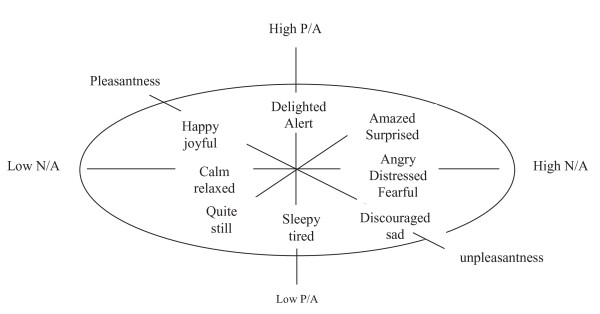
\includegraphics[width=\linewidth]{images/tellegen-watson-clark-model.jpg}
	\centering
	\textbf{The Tellegen-Watson-Clark model of mood} \citep{Tellegen1999}
\end{Figure}

\subsection{Feature Extraction and Classification}
Different researchers have tried different approaches to classification of music, not necessarily for classification of emotion. \citet{Mckinney2003} have proposed a method to automatically determine the genre of a certain piece of audio, including noise and speech. They tested different methods of classification against each other, resulting in good values for MFCC Analysis as well as Psychoacoustic features and a set of features called auditory filter temporal envelope, a set of bandpass filters which mimics the range of hearing of a human ear.\\

\citet{Li2003} give a comparison of classification techniques for automatic assignment of genres, including MFCC, FFT, Beat and Pitch, showing best results for FFT and MFCC, or a combination of these with other features. They make use of a Support Vector Machine for classifying, with good results.
\citet{Tzanetakis2001} also focus on the automatic classification of genres, focusing on the calculation of certain features such as STFT (short time fourier transform) and MFCC. The paper shows how to calculate the different features and explains the results. They find the best results when working with MFCC and STFT and identify genres that are harder to distinguish than others.

\section{Emotion Model}
To be able to distinguish between emotions more easily, we decided to use a simplified version of the Tellegen-Watson-Clark model. We defined four emotional categories, marking the extreme ends of the graphs used in the model. The categories proposed in the Tellegen-Watson-Clark model have some adjectives that are very similar and difficult to distinguish especially when dealing with music as a carrier of emotion. Categories such as \textit{calm-relaxing} and \textit{quiet-still}, or \textit{amazed-surprised} and \textit{happy-pleased} were combined into one category. The remaining categories are:

\begin{itemize}
	\item calm-relaxing
	\item happy-amazed
	\item angry-fearful
	\item sad-lonely
\end{itemize}

\section{Training Data}\label{training-data}
To create a the training data for the classifier, we accumulated a collection of 424 songs of various genre and artist, roughly sorted by their main emotion, by searching various online streaming and video platforms, such as Youtube and Spotify for playlists with tags fitting our emotional model.\\
Those songs were then tagged by 3 independent raters into the four emotional categories mentioned above. Afterwards \textit{Fleiss' Kappa} was calculated over the results, to use only songs for the creation of the training data where all raters agreed on the same emotion. The following table schows the distribution of kappa values over all songs.\\

\begin{center}
\label{kappa-distribution}
\begin{tabular}{@{}lll@{}}
Kappa & Count & Percent \\ \midrule
1.00 & 260 & 61.32\% \\
0.33 & 155 & 36.56\% \\
0.00 & 9 	 & 2.12\%
\end{tabular}
\end{center}

Most of the disagreement (90 songs) were in categories \textit{calm-relaxing} and \textit{sad-lonely}, predicting difficulties in the differentiation of these categories.\\

To try to get an overview about useful features we processed a small sample of audio files with the jAudio feature extractor \citep{McEnnis2005}, extracting as many features as possible. We then used a two-step cluster analysis to analyse which features were actually usable for classification. We found out that the MFCC, along with several low level features, such as RMS, were showing promising results and decided to use these features for the classification. Previous research on wich features to use for audio classification has shown similar results \citep{Mckinney2003, Mandel2005, Tzanetakis2001}. Because the application is meant to be used in real time, the feature extraction needs to be as quickly as possible. Therefore as little features as possible were used without impairing the classification too much. The final feature vector consists of 26 features.

\begin{center}
\begin{tabular}{@{}ll@{}}
Feature Count & Feature Name \\ \midrule
13 & MFCC \\
12 & Chroma \\
1  & RMS
\end{tabular}
\end{center}

\section{System}
During the development of the feature extraction process several approaches were tested for performance and format compatibility. Since the audio processing library \textit{MARSYAS} \citep{Tzanetakis1999} is written in C++ it was not considered for the player. \textit{TarsosDSP} \citep{Six2014} is another audio processing library with focus on real time audio processing. It is written in Java but does not support the mp3 format. The last library considered was \textit{jAudio} \citep{McEnnis2005}, a gui application specifically developed for feature extraction. This application is also written in Java and supports both wav and mp3 formats and was therefore chosen over the other two.\\

The system was realized as a simple Music Player. The user interface provides a set of buttons associated with the emotions, which allow the user to filter the available songs by their emotion. A song is classified as soon as it is loaded into the music library of the player.

\begin{Figure}
	\label{screenshot}
	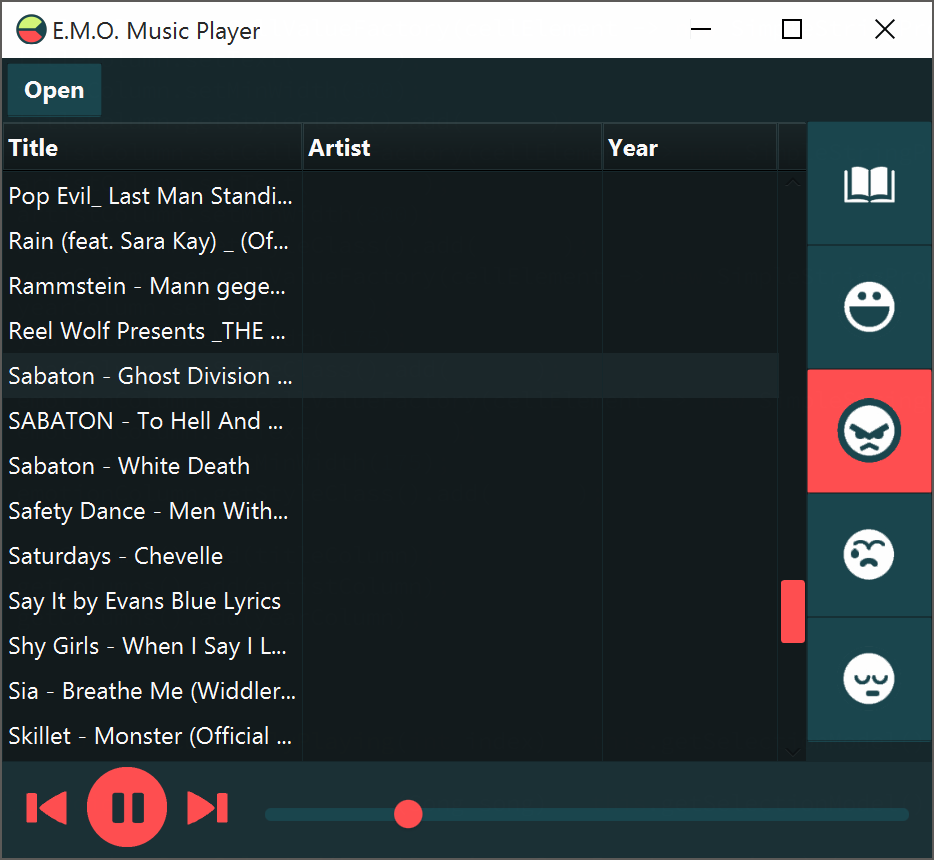
\includegraphics[width=\linewidth]{images/screenshot.png}
	\centering
	\textbf{User interface of the music player}
\end{Figure}
\vspace*{5pt}

The classification is done by a Naive Bayes classifier, because it showed the best performance in comparison to the other classifiers tested (Support Vector Machine, Logistic Regression, Decision Trees).

\section{Results}
The classifier was trained using the training data explained in \ref{training-data} and evaluated using 10-fold cross validation. The classifier seems to perform poorly given that only 54.07\% of all songs could be correctly classified, but having in mind that human raters assigned to only 61.32\% of all songs the same label, the classifier performs very well. The results also show, that the emotion of a song is a highly subjective experience and may need additional input data, like analysis of lyrics or additional audio features to become more precisely determinable.

\begin{center}
\begin{tabular}{@{}lll@{}}
\multicolumn{3}{c}{\textbf{Naive Bayes Classification Results}} \\ \midrule
Correctly Classified             & 138      & 53.07\% \\
Incorrectly Classified           & 122      & 46.92\% \\
Kappa statistic 				 & 0.35     & \\
Mean absolute error  			 & 0.23     & \\
Root mean squared error 		 & 0.45     & \\
Relative absolute error 		 & 64.52\%  & \\
Root relative squared error 	 & 105.10\% & \\
Total Number of Instances 		 & 260      & 100\%
\end{tabular}
\end{center}

In the process of the project, we have come to a few conclusions regarding methods and tools. We used the jAudio library to get an overview of available features, but struggled with the documentation of the code during the implementation. While jAudio has an easy to use graphical user interface for feature extraction, which can create great amounts of usable data in little time, the possibility to embed the application into a system is lacking.

\section{Conclusion}
We found that it is possible to classify music via emotion and build a recommending system around that classification. With further refinement of the extracted features and possibly the addition of non-musical features such as lyrics, we are positive that the accuracy of the classification can be further improved. A recommendation system such as this could, for example, be trained on the large library of a streaming platform and built into the player, as a new and unique way to find music.

\bibliographystyle{apacite}
\bibliography{literature}

\end{multicols}
\end{document}
